\part{Model Based Design of Control Systems}

\chapter{Introduction}

\section{Adaptive cruise control example}

\begin{itemize}
	\item Specification: Maintain constant velocity against road gradients
	\item Control Signal: Throttle angle
	\item Disturbance: Road-gradient
	\item Output: Velocity
\end{itemize}

The relationship between control input $u$ and system output $v$ can be modeled using Newtons laws as described below:
\begin{equation}\label{Eq_ACC_PlantModel}
	\frac{dv}{dt} = -\frac{a}{m}v + \frac{b}{m}
\end{equation}

Adding disturbance to plant model given by equation \eqref{Eq_ACC_PlantModel} the following system model can be described:
\begin{equation} \label{Eq_ACC_PlantModel_with_d}
	\frac{dv}{dt} = -\frac{a}{m}v + \frac{b}{m} -d
\end{equation}
where $d = g sin(\alpha)$ and $\alpha$ is the road-gradient.

\subsection{Open-loop control design}

The system model given by equation \eqref{Eq_ACC_PlantModel} can be expressed in LT from as:
\begin{equation}
	G(s) = \frac{V(s)}{U(s)} = \frac{b/m}{s + a/m}
\end{equation}

In order to determine the OL control input, an assumption is made such that $\alpha = 0$, the control input is then:
\begin{equation}
	0 = -\frac{a}{m}v + \frac{b}{m} \implies u = \frac{a}{b} r
\end{equation}
where $r = v$, as velocity is supposed to follow the reference. $u$ is LT will be:
\begin{equation} \label{Eq_ACC_OL_ControlSignal}
	U(s) = \frac{a}{b}R(s)
\end{equation}
As described in section \ref{Sec_OL_ControlArchitecture}, the OL control signal is inverse of the plane $P(s)$, from equation \eqref{Eq_ACC_OL_ControlSignal} it can be seen that at steady-state $s \rightarrow 0$, $P(s) = b/a$. The system model with control input is as shown in figure \ref{Fig_ACC_OL_control}.
\begin{figure}[h!]
	\centering
	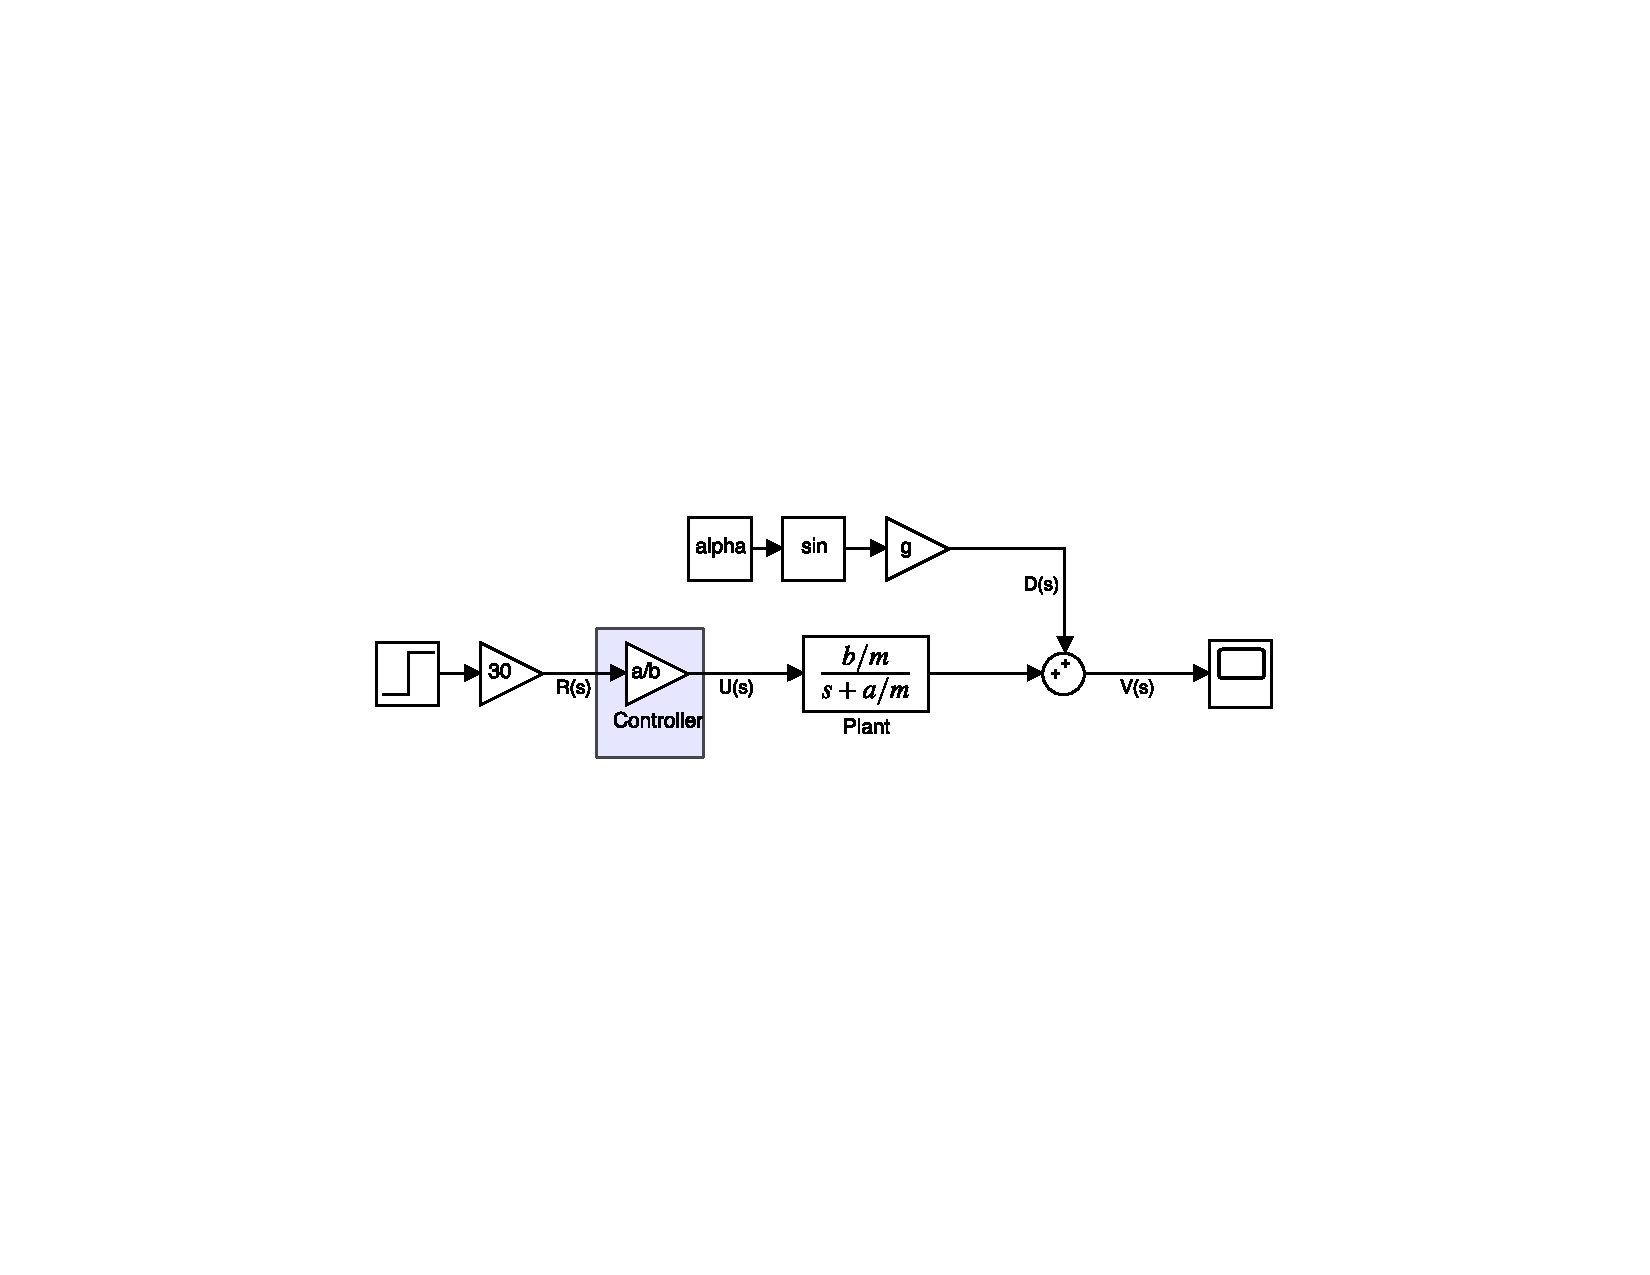
\includegraphics[width=\linewidth]{Bilder/ACC_OL}
	\caption{ACC in OL control}
	\label{Fig_ACC_OL_control}
\end{figure}
The response of the system shown in figure \ref{Fig_ACC_OL_control} is shown in figure \ref{Fig_ACC_OL_control_Response}. It can be seen that for no $D(s)$, the system follows $R(s)$.
\begin{figure}[h!]
	\centering
	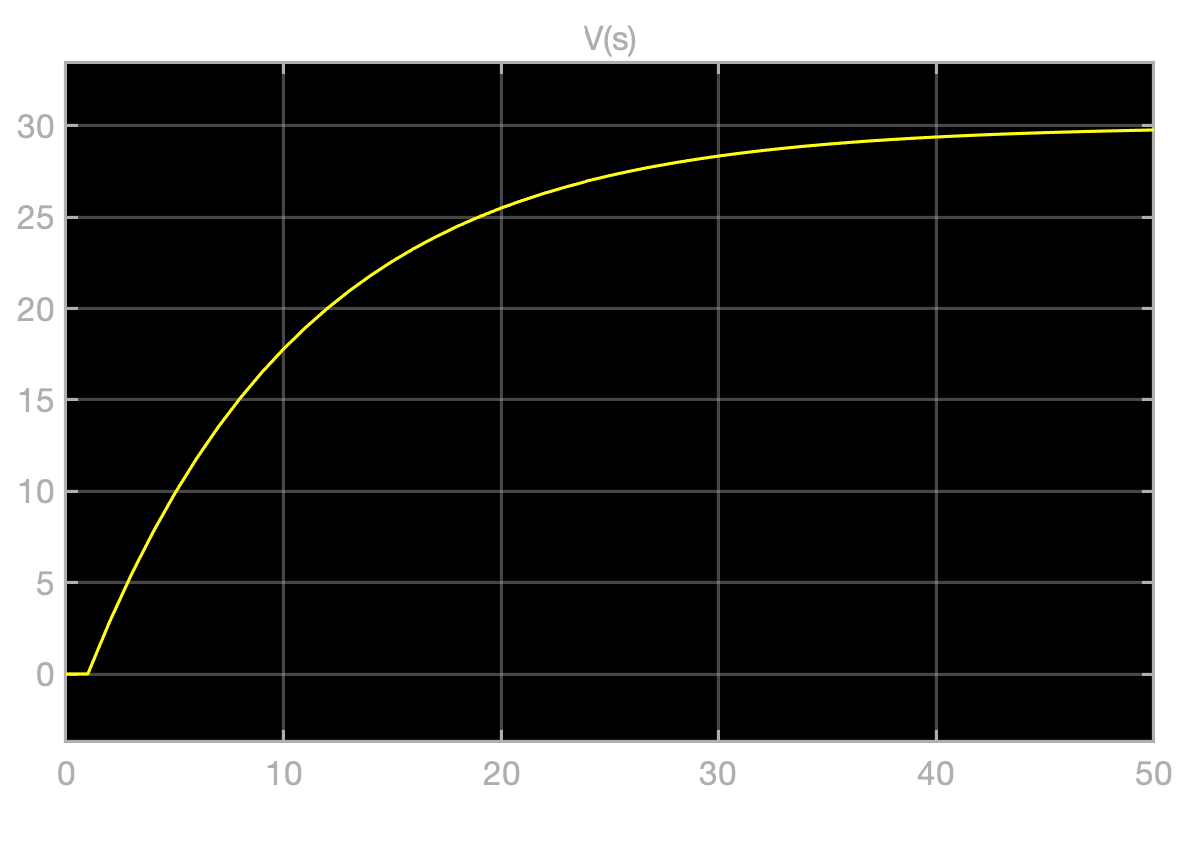
\includegraphics[width=0.7\linewidth]{Bilder/ACC_OL_response.eps}
	\caption{ACC in OL control}
	\label{Fig_ACC_OL_control_Response}
\end{figure}
Generally, OL system cannot track changes in road-gradient and changes in system parameters, since the control signal given by \eqref{Eq_ACC_OL_ControlSignal} eliminates system parameters, the control has become robust in my case for any change in road-gradient and/or the system parameter $m$. However, if other system parameters $(a, \quad b)$ are not predefined in the control, the system would not following the reference properly. Also note that from figure \ref{Fig_ACC_OL_control_Response}, the system is quite sluggish, as it is very slow to settle for a given input $R(s)$. These two problems could be solved using a feedback controller.

\section{Model Based Control Design general methodology}

Control design technology based on Model Based Design is very important in Automotive development. Some of the examples are Power-train control, Engine control, ABS and more advanced controls used in Autonomous driving such as Lane assist, Tracking etc.,. The following general methodology is used in control system design in Automotive applications:
\begin{enumerate}
	\item Control objectives (specification)
	\begin{enumerate}
		\item Asks questions on what should be established using a control
		\item Requires knowledge on system dynamics as well as disturbances, so that a valid performance could be achieved and not fight the system against it own
		\item Kinds of control objectives:
		\begin{enumerate}
			\item \textbf{Qualitative objectives}: Objectives that are listed as some kind of improvements that are not exactly specified (achieving as good results as possible) such as some improvement in fuel-consumption, minimize battery energy consumption etc.,
			\item \textbf{Quantitative objectives}: Objectives that are well-defined such as achieving desired response times
		\end{enumerate}
	\end{enumerate}
	\item Description of system or a plant
	\begin{enumerate}
		\item Asks questions on level of system abstraction required (component level, subsystem level or plant level etc.,)
		\item Modeling can be done in various ways such as mathematical or measurements (black-box) etc.,
	\end{enumerate}
	\item Controller Design
	\begin{enumerate}
		\item Up until plant model, the system is on the HW side, from controller design onward, the SW side of the system developments starts
		\item Asks questions on type of control design such as OL or CL etc.,
		\item Several design methods are employed such as classical methods (PID) or modern methods using state-space methods
		\item Choosing control parameters is most important which will determine the performance of the system. mostly methods such as trail and error, design methods from control theory and optimization methods are employed
	\end{enumerate}
	\item Analyze the performance: To check if the desired results are achieved, methods that are used are:
	\begin{enumerate}
		\item Analysis
		\item Simulation
		\item Experiments (Testing)
	\end{enumerate}
\end{enumerate}

\section{Control design methods}
\textbf{\textit{Classical control design (PID)}}
\begin{enumerate}
	\item Works well for simple systems
	\item Do not require good mathematical knowledge of the systems as the controller parameters can be designed using trail and error methods
	\item A good control theory knowledge can also be helpful for better design but are rather intensive
	\item Due to their large trail and error iterations this method is mot ideal for system with multiple input and outputs (MIMO)
\end{enumerate}

\textbf{\textit{State-space method}}
\begin{enumerate}
	\item can easily handle large scale systems (MIMO)
	\item tuning can be formed as an optimization problem and are available as systematic tools that are pre-developed
	\item they are also easier to implement
	\item on the other hand state-space control design requires good mathematical knowledge
\end{enumerate}

\section{State-space control design methodology}

State-space methods for a control design is a very powerful technique for a control design because they are very systematic and not based on theoretical intuition required in classical control design. This method is best suited for large scale systems such as an Automotive but are seldom taught in a formalized way in most of the control courses. 

A state-space is a dynamic modeling of a system using first order differential or difference equations. The state-space methodology can be visualized using the figure \ref{Fig_StateSpaceMethodology}.
\begin{figure}[h!]
	\centering
	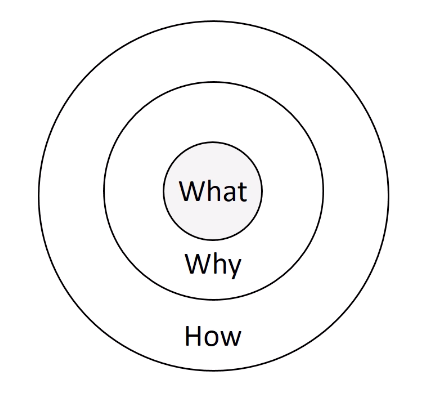
\includegraphics[width=0.7\linewidth]{Bilder/StateSpaceMethodology}
	\caption{Visualizing state space modeling}
	\label{Fig_StateSpaceMethodology}
\end{figure}

The what of state-space model is the description of the system dynamics using first order differential or difference equations, here state variables are used that essentially are sufficient to describe the evolution of the system. They are regarded as the memory of the system which remembers the past and acts based on it in the present and the future. A state-space form is expressed as:
\begin{align}
	\dot{x}(t) &= f(x(t),u(t)) \\
	y(t) &= h(x(t),u(t))
\end{align}
A special case of state-space form is autonomous (as described above) and linear system which is expressed as linear combinations of state vectors and input vectors as expressed below:
\begin{align}
	\dot{x} &= A x + B u \\
	y &= Cx + Du
\end{align}

The why part describes why should one use state-space modeling approach:
\begin{enumerate}
	\item They are natural for modeling physical systems
	\item are easy to use due to matrix format
	\item also makes it great to use for MIMO systems (which are hard to use with LT's)
	\item easy to implement for ex: the control equation $u = Lx + Kr$ is a one line code which contains simple vector or matrix algebra
\end{enumerate}

The how part deals with how the state space model can be implemented from development phase to implementation phase, the general method is as follows:
\begin{enumerate}
	\item Modeling
	\item Analysis (For system knowledge)
	\item Controller design (State Feedback controller)
	\item Observer / Estimator design: To measure the required states used for state feedback controller. Generally, in a system measuring required states is not direct and easy but with state space method there are tools available that makes it possible to do so
\end{enumerate}